\section{Конструкторская часть}

В данном разделе будут рассмотрены возможные сценарии неправомерных действий и признаки, по которым данные неправомерные действия могут быть обнаружены, будет рассмотрена функциональная схема программного комплекса, а также будет рассмотрен алгоритм обновления хеш-сумм для связи всех звеньев.

\subsection{Сценарии неправомерных действий}

На рисунке \ref{fig:scenarios} изображены сценарии возможного неправомерного доступа. Здесь рассматриваются только действия с данными, без метаданных.

\begin{figure}[hbtp]
	\centering
	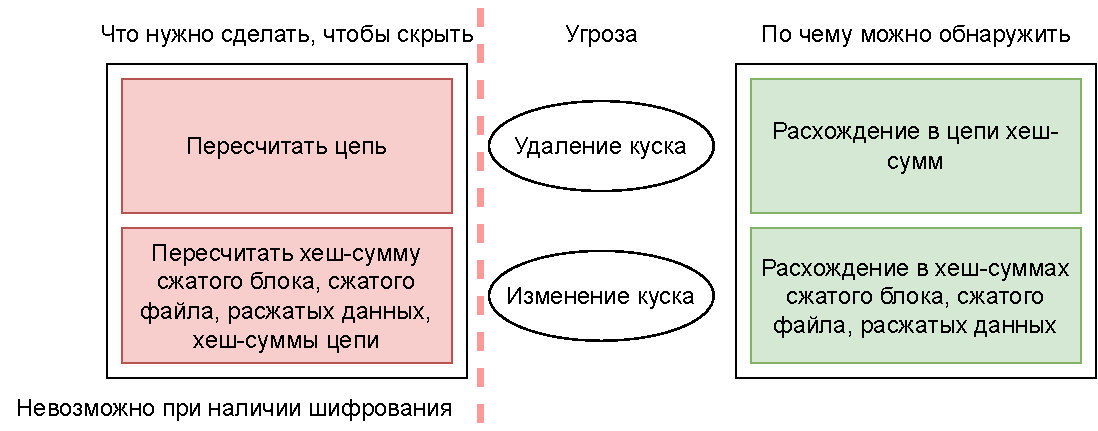
\includegraphics[width=\textwidth]{img/scenarios.pdf}
	\caption{Сценарии неправомерных действий.}
	\label{fig:scenarios}
\end{figure}

\subsection{Функциональная схема программного комплекса}

На рисунке \ref{fig:idef} представлена функциональная схема разрабатываемого программного комплекса.

\begin{figure}[hbtp]
	\centering
	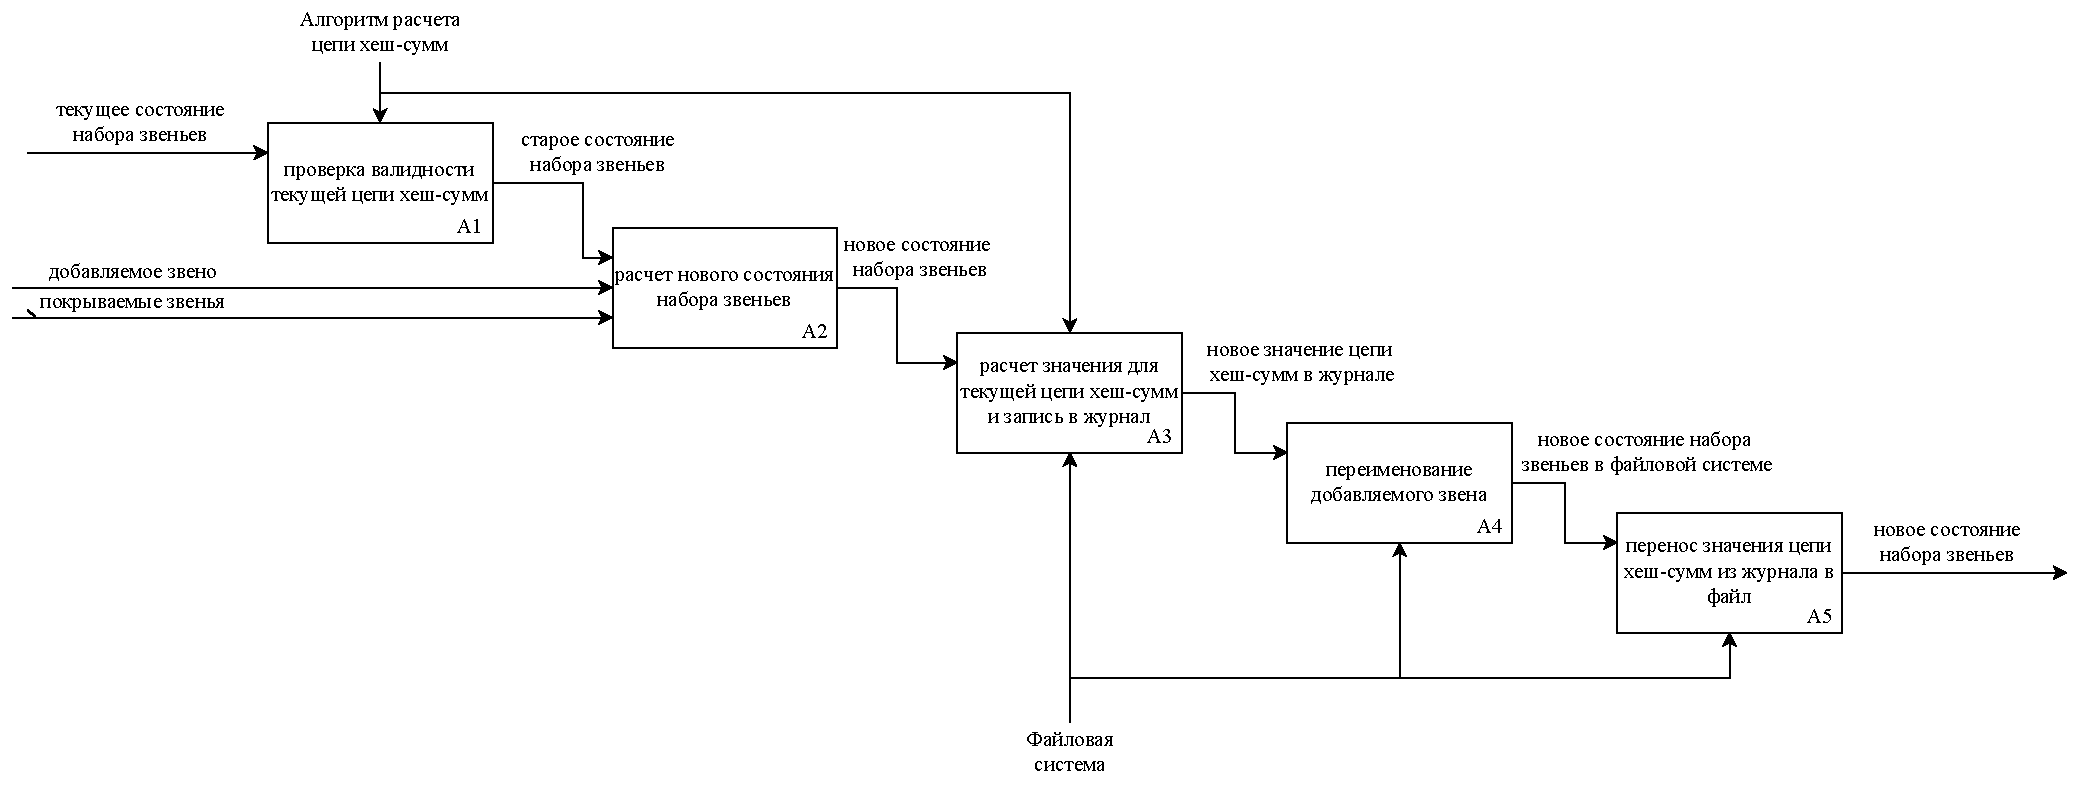
\includegraphics[width=\textwidth]{img/idef.pdf}
	\caption{Функциональная схема программного комплекса.}
	\label{fig:idef}
\end{figure}

\subsection{Схемы алгоритмов работы метода}

На рисунках \ref{fig:mainalgo} и \ref{fig:mainalgo2} показана схема нового алгоритма изменения состояний звеньев. Серым отмечены блоки, которые присутствовали в старом алгоритме. Во внутренней структуре состояния звеньев меняются следующим образом:
\begin{itemize}
	\item [---] звено, который переименовывается из временного в обычный, переходит из временного состояния в активное;
	\item [---] звенья, которые покрываются переименовываемым звеном, переводятся из активного состояния в истекшее и не используются при чтении.
\end{itemize}

На рисунке \ref{fig:recalcalgo} показана схема алгоритма расчета цепи хеш-сумм.

На рисунке \ref{fig:checkalgo} показана схема алгоритма проверки цепи хеш-сумм.


\begin{figure}[hbtp]
	\centering
	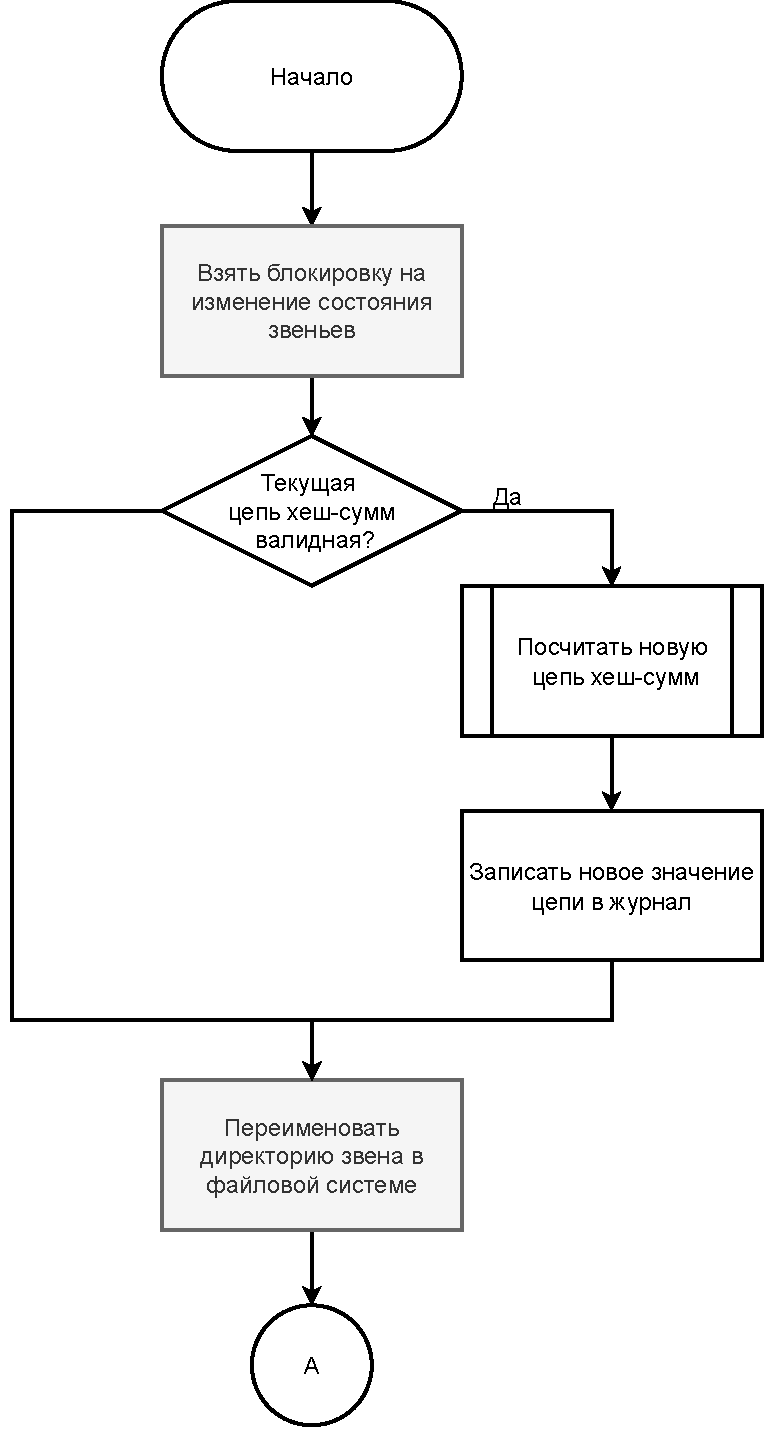
\includegraphics[scale=0.8]{img/mainalgo.pdf}
	\caption{Схема нового алгоритма изменения состояний звеньев.}
	\label{fig:mainalgo}
\end{figure}
\begin{figure}[hbtp]
	\centering
	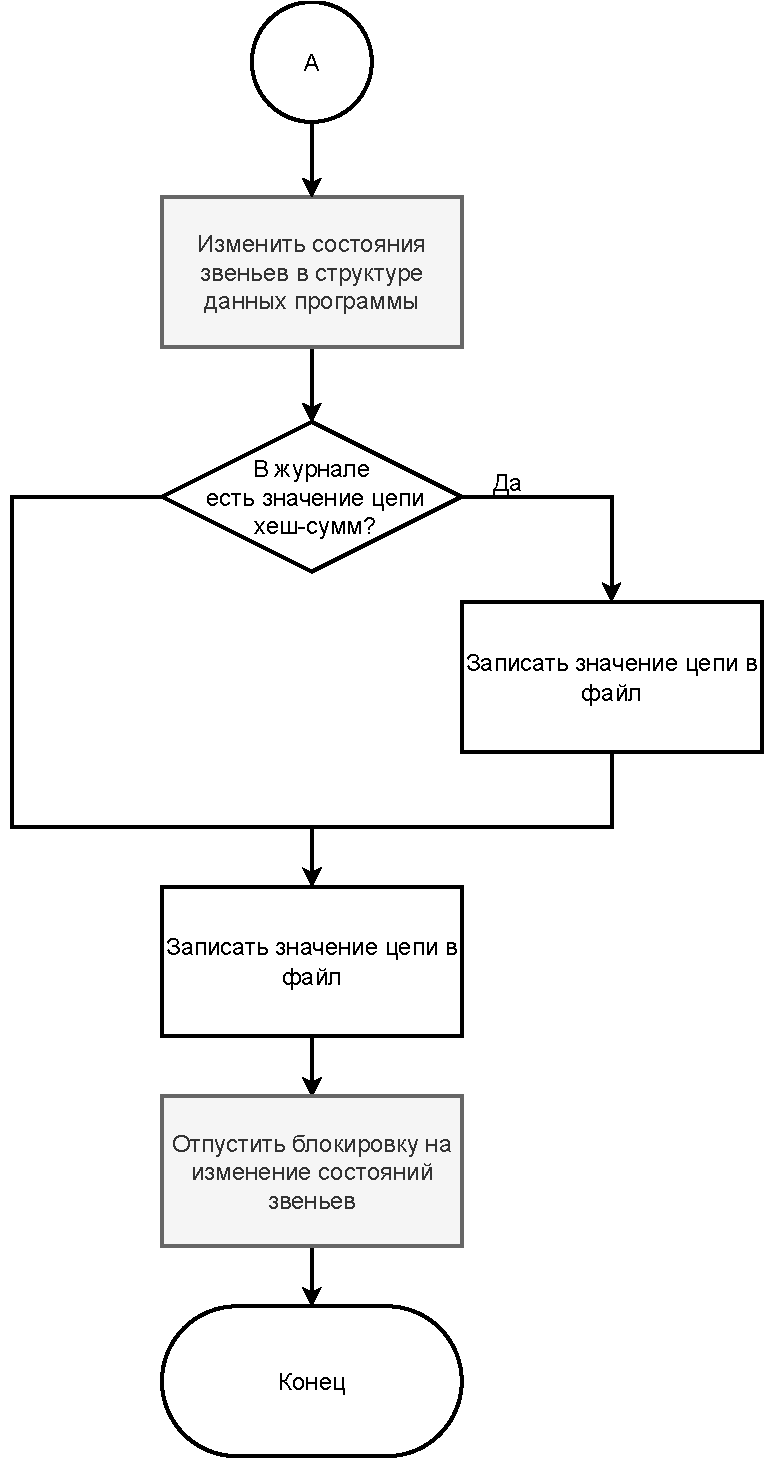
\includegraphics[scale=0.8]{img/mainalgo2.pdf}
	\caption{Схема нового алгоритма изменения состояний звеньев. Продолжение.}
	\label{fig:mainalgo2}
\end{figure}

\begin{figure}[hbtp]
	\centering
	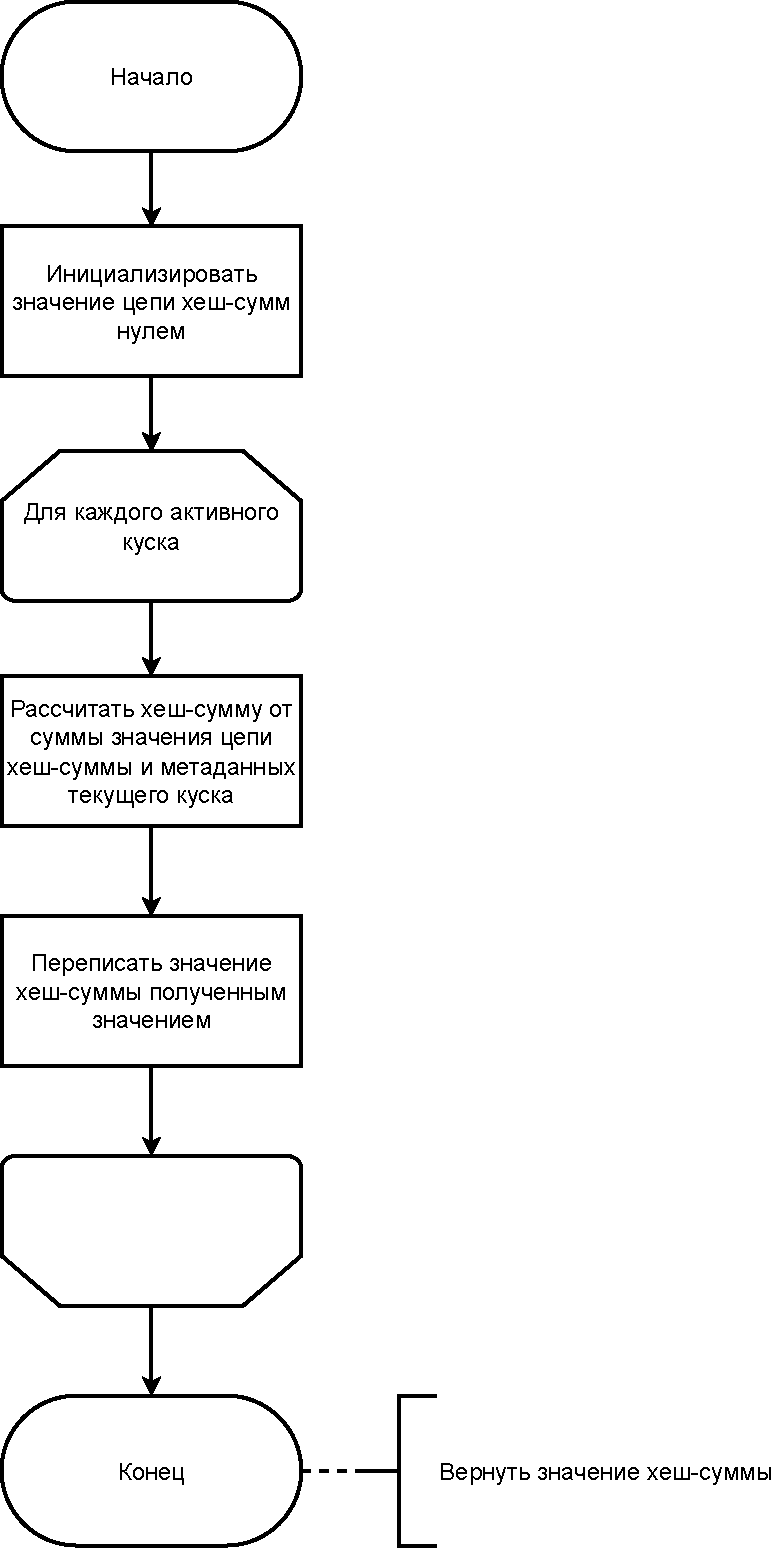
\includegraphics[scale=0.8]{img/recalcalgo.pdf}
	\caption{Схема алгоритма расчета цепи хеш-сумм.}
	\label{fig:recalcalgo}
\end{figure}

\begin{figure}[hbtp]
	\centering
	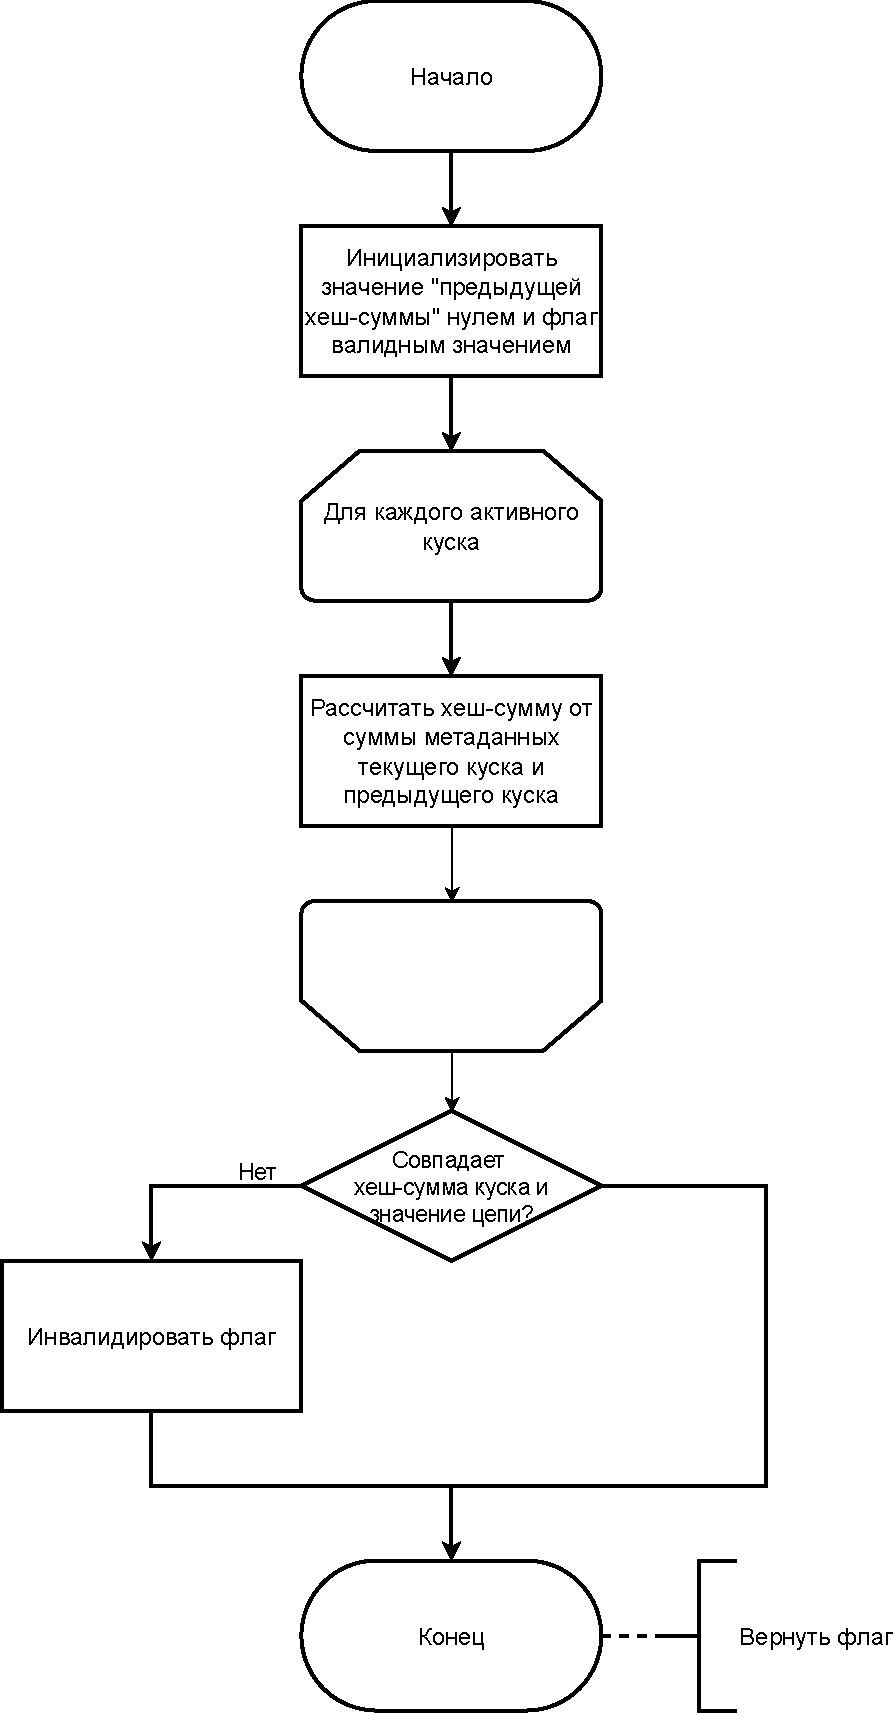
\includegraphics[scale=0.75]{img/checkalgo.pdf}
	\caption{Схема алгоритма проверки валидности цепи хеш-сумм.}
	\label{fig:checkalgo}
\end{figure}

\subsection{Выводы}

В данном разделе были рассмотрены возможные сценарии неправомерного доступа, а также построены схемы алгоритмов, необходимых для реализации разрабатываемого метода.

\pagebreak